% RNNs and LSTM

\begin{slide}{Sequences}
  \begin{itemize}
    \item<1-> Humans think in sequences
    \item<2-> Simple neural networks don't
    \item<3-> Sequences give single entities context
    \item<5-> The key to understanding sequences is memory
  \end{itemize}
  \vspace{0.5cm}

  \onslide<3->{I }\onslide<4->{enjoy }\onslide<3->{eat}\onslide<4->{ing dinner with }\onslide<3->{people}
\end{slide}

\begin{slide}{Machine Memory}
  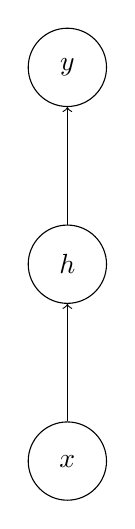
\begin{tikzpicture}
    % Nodes
    \path (0, 0) coordinate [draw, circle, inner sep=10pt] (x) node {$x$};
    \path (0, 2.5) coordinate [draw, circle, inner sep=10pt] (h) node {$h$};
    \path (0, 5) coordinate [draw, circle, inner sep=10pt] (y) node {$y$};

    % Connections
    \draw [->] (x) -- (h);
    \draw [->] (h) -- (y);
  \end{tikzpicture}
\end{slide}

\begin{frame}[fragile]{Machine Memory}
  \begin{center}
  \begin{tikzpicture}
    % Nodes
    \path (0, 0) coordinate [draw, circle, inner sep=10pt] (x) node {$x_t$};
    \path (0, 2.5) coordinate [draw, circle, inner sep=10pt] (h) node {$h_t$};
    \path (0, 5) coordinate [draw, circle, inner sep=10pt] (y) node {$y_t$};

    % Connections
    \draw [->] (x) -- (h);
    \draw [->] (h) -- (y);

    \newcommand{\timestep}[2]{
      % Nodes
      \path (#1, 0) coordinate [draw, circle, inner sep=10pt]
            (x#2) node {$x_{t+#2}$};
      \path (#1, 2.5) coordinate [draw, circle, inner sep=10pt]
            (h#2) node {$h_{t+#2}$};
      \path (#1, 5) coordinate [draw, circle, inner sep=10pt]
            (y#2) node {$y_{t+#2}$};

      % Connections
      \draw [->] (x#2) -- (h#2);
      \draw [->] (h#2) -- (y#2);
    }

    \only<2> {
      \draw [->] (h) [out=45,in=-45,looseness=5] to (h);
      \draw (1.6, 2.5) node {$h_{t-1}$};
    }

    \only<3-> {
      \timestep{2}{1}
      \draw [->] (h) -- (h1);
    }
    \only<4-> {
      \timestep{4}{2}
      \draw [->] (h1) -- (h2);
    }
    \only<5-> {
      \timestep{6}{3}
      \draw [->] (h2) -- (h3);
    }
    \only<6-> {
      \timestep{8}{4}
      \draw [->] (h3) -- (h4);
    }
  \end{tikzpicture}
  \end{center}
\end{frame}

\begin{slide}{Machine Memory}
  $$h_t = f(w \cdot x + b)$$
\end{slide}

\begin{slide}{Machine Memory}
  $$h_t = f(\mathbf{w}^\top [h_{t-1}, x] + b)$$
\end{slide}

\begin{slide}{Recurrent Neural Networks}
  \begin{itemize}
    \item Recurrent Neural Networks (RNNs) share weights through time
    \item They have \emph{memory}
    \item And they have a problem:
  \end{itemize}
  \vspace{1cm}
  {
    \Large
    The Vanishing Gradient Problem
  }
\end{slide}

% \begin{frame}[fragile]{Machine Memory}
%   \begin{center}
%   \begin{tikzpicture}
%     % Nodes
%     \path (0, 0) coordinate [draw, circle, inner sep=10pt] (x) node {$x_t$};
%     \path (0, 2.5) coordinate [draw, circle, inner sep=10pt] (h) node {$h_t$};
%     \path (0, 5) coordinate [draw, circle, inner sep=10pt] (y) node {$y_t$};
%
%     % Connections
%     \only<1>{\draw [->] (x) -- (h);}
%     \only<2>{\draw [->] (x) -- (h) node [left, midway] {$w$};}
%     \draw [->] (h) -- (y);
%
%     \newcommand{\timestep}[2]{
%       % Nodes
%       \path (#1, 0) coordinate [draw, circle, inner sep=10pt]
%             (x#2) node {$x_{t+#2}$};
%       \path (#1, 2.5) coordinate [draw, circle, inner sep=10pt]
%             (h#2) node {$h_{t+#2}$};
%       \path (#1, 5) coordinate [draw, circle, inner sep=10pt]
%             (y#2) node {$y_{t+#2}$};
%
%       % Connections
%       \only<1>{\draw [->] (x#2) -- (h#2);}
%       \only<2->{\draw [->] (x#2) -- (h#2) node [left, midway] {$w$};}
%       \draw [->] (h#2) -- (y#2);
%     }
%
%     \timestep{2}{1}
%     \draw [->] (h) -- (h1);
%
%     \timestep{4}{2}
%     \draw [->] (h1) -- (h2);
%   \end{tikzpicture}
%   \end{center}
% \end{frame}
%
% \begin{frame}[fragile]{Machine Memory}
%   \begin{center}
%   \begin{tikzpicture}
%     % Nodes
%     \path (0, 0) coordinate [draw, circle, inner sep=10pt] (x) node {$x_t$};
%     \path (0, 2.5) coordinate [draw, circle, inner sep=10pt] (h) node {$h_t$};
%     \path (0, 5) coordinate [draw, circle, inner sep=10pt] (y) node {$y_t$};
%     \path (0, 1.25) coordinate [draw, circle, inner sep=7pt]
%           (w) node {$w$};
%
%     % Connections
%     \draw [->] (x) -- (w);
%     \draw [->] (w) -- (h);
%     \draw [->] (h) -- (y);
%
%     \newcommand{\timestep}[2]{
%       % Nodes
%       \path (#1, 0) coordinate [draw, circle, inner sep=10pt]
%             (x#2) node {$x_{t+#2}$};
%       \path (#1, 2.5) coordinate [draw, circle, inner sep=10pt]
%             (h#2) node {$h_{t+#2}$};
%       \path (#1, 5) coordinate [draw, circle, inner sep=10pt]
%             (y#2) node {$y_{t+#2}$};
%       \path (#1, 1.25) coordinate [draw, circle, inner sep=7pt]
%             (w#2) node {$w$};
%
%       % Connections
%       \draw [->] (x#2) -- (w#2);
%       \draw [->] (w#2) -- (h#2);
%       \draw [->] (h#2) -- (y#2);
%     }
%
%     \timestep{2}{1}
%     \draw [->] (h) -- (h1);
%
%     \timestep{4}{2}
%     \draw [->] (h1) -- (h2);
%   \end{tikzpicture}
%   \end{center}
% \end{frame}
%
% \begin{frame}[fragile]{Machine Memory}
%   \begin{center}
%   \begin{tikzpicture}
%     % Nodes
%     \path (0, 0) coordinate [draw, circle, inner sep=10pt] (x) node {$x_t$};
%     \path (0, 2.5) coordinate [draw, circle, inner sep=10pt] (h) node {$h_t$};
%     \path (0, 5) coordinate [draw, circle, inner sep=10pt] (y) node {$y_t$};
%     \path (0, 1.25) coordinate [draw, circle, inner sep=7pt]
%           (w) node {$w$};
%
%     % Connections
%     \draw [->] (x) -- (w);
%     \draw [->] (w) -- (h);
%     \draw [->] (h) -- (y);
%
%     \newcommand{\timestep}[2]{
%       % Nodes
%       \path (#1, 0) coordinate [draw, circle, inner sep=10pt]
%             (x#2) node {$x_{t-#2}$};
%       \path (#1, 2.5) coordinate [draw, circle, inner sep=10pt]
%             (h#2) node {$h_{t-#2}$};
%       \path (#1, 5) coordinate [draw, circle, inner sep=10pt]
%             (y#2) node {$y_{t-#2}$};
%       \path (#1, 1.25) coordinate [draw, circle, inner sep=7pt]
%             (w#2) node {$w$};
%
%       % Connections
%       \draw [->] (x#2) -- (w#2);
%       \draw [->] (w#2) -- (h#2);
%       \draw [->] (h#2) -- (y#2);
%     }
%
%     \timestep{-2}{1}
%     \draw [->] (h) -- (h1);
%
%     \timestep{-4}{2}
%     \draw [->] (h1) -- (h2);
%   \end{tikzpicture}
%   \end{center}
% \end{frame}
%
% \begin{frame}[fragile]{Machine Memory}
%   \begin{center}
%   \begin{tikzpicture}
%     % Nodes
%     \path (0, 2.5) coordinate [draw, circle, inner sep=10pt] (h) node {$h_t$};
%     \path (0, 5) coordinate [draw, circle, inner sep=10pt] (y) node {$y_t$};
%     \path (0, 1.25) coordinate [draw, circle, inner sep=7pt]
%           (w) node {$w$};
%
%     % Connections
%     \draw [->] (w) -- (h);
%     \draw [->] (h) -- (y);
%
%     \newcommand{\timestep}[2]{
%       % Nodes
%       \path (#1, 2.5) coordinate [draw, circle, inner sep=10pt]
%             (h#2) node {$h_{t-#2}$};
%       \path (#1, 1.25) coordinate [draw, circle, inner sep=7pt]
%             (w#2) node {$w$};
%
%       % Connections
%       \draw [->] (w#2) -- (h#2);
%     }
%
%     \timestep{-2}{1}
%     \draw [->] (h) -- (h1);
%
%     \timestep{-4}{2}
%     \draw [->] (h1) -- (h2);
%   \end{tikzpicture}
%   \end{center}
% \end{frame}
%
% \begin{frame}[fragile]{Machine Memory}
%   \begin{center}
%   \begin{tikzpicture}
%     % Weight
%     \path (-2, 0) coordinate [draw, circle, inner sep=7pt]
%           (w) node {$w$};
%
%     % Nodes
%     \path (0, 2.5) coordinate [draw, circle, inner sep=10pt] (h) node {$h_t$};
%     \path (0, 5) coordinate [draw, circle, inner sep=10pt] (y) node {$y_t$};
%
%     % Connections
%     \only<1>{\draw [->] (h) -- (y);}
%     \only<2->{
%       \draw [red, ->] (h) -- (y)
%             node [black, right, midway] {$\frac{\partial y_t}{\partial h_t}$};
%     }
%     \only<-2>{\draw [->] (w) -- (h);}
%     \only<3->{
%       \draw [red, ->] (w) -- (h)
%             node [black, right, pos=0.7] {$\frac{\partial h_t}{\partial w}$};
%     }
%
%     % Nodes
%     \path (-2, 2.5) coordinate [draw, circle, inner sep=10pt]
%           (h1) node {$h_{t-1}$};
%     % Connections
%     \only<-4>{\draw [->] (w) -- (h1);}
%     \only<5->{
%       \draw [red, ->] (w) -- (h1)
%             node [black, right, pos=0.7] {$\frac{\partial h_{t-1}}{\partial w}$};
%     }
%     \only<-3>{\draw [->] (h) -- (h1);}
%     \only<4->{
%       \draw [red, ->] (h) -- (h1)
%             node [black, above, midway] {$\frac{\partial h_t}{\partial h_{t-1}}$};
%     }
%
%     \path (-4, 2.5) coordinate [draw, circle, inner sep=10pt]
%           (h2) node {$h_{t-2}$};
%     % Connections
%     \only<-6>{\draw [->] (w) -- (h2);}
%     \only<7->{
%       \draw [red, ->] (w) -- (h2)
%             node [black, pos=0.7, right] {$\frac{\partial h_{t-2}}{\partial w}$};
%     }
%     \only<-5>{\draw [->] (h1) -- (h2);}
%     \only<6->{
%       \draw [red, ->] (h1) -- (h2)
%             node [black, above, midway] {$\frac{\partial h_{t-1}}{\partial h_{t-2}}$};
%     }
%
%     \only<7-> {
%     \path (-7, 2.5) coordinate [draw, circle, inner sep=10pt]
%           (1) node {$h_1$};
%       \draw [semithick, dotted, ->] (h2) -- (1);
%       \draw [->] (w) -- (1);
%     }
%     \onslide<8>{
%     \draw (-3, -1) node {%
%       $
%         \frac{\partial h_t}{\partial h_{t-1}}
%         \frac{\partial h_{t-1}}{\partial h_{t-2}}
%         \frac{\partial h_{t-2}}{\partial h_{t-3}}
%         \dotsm
%         \frac{\partial h_2}{\partial h_1}
%       $
%     };
%     }
%     \onslide<9>{
%       \draw (-3, -1) node {$0.1 \cdot 0.1 \cdot 0.1 \dotsm 0.1$};
%     }
%     \onslide<10>{
%       \draw (-3, -1) node {$0.1 \cdot 0.1 \cdot 0.1 \dotsm 0.1 \approx 0$};
%     }
%   \end{tikzpicture}
%   \end{center}
% \end{frame}

\begin{slide}{LSTMs}
  \begin{itemize}
    \item<1-> RNN's are forgetful
    \item<2-> \emph{Long Short Term Memory} (LSTM) Units solve this problem
    \item<3-> Developed by Schmidhuber and Hochreiter at TUM in 1997
  \end{itemize}
\end{slide}

% First explain what an LSTM consists of

\begin{slide}{LSTMs}
  \begin{itemize}
    \pitem LSTMs are a lot like flip-flops
    \pitem They have three \emph{gates}
    \begin{itemize}
      \pitem Input gate $G_i(x, h_{t-1}) = \sigma(\mathbf{w}_i^\top [x, h_{t-1}] + b_i)$
      \pitem Forget gate $G_f(x, h_{t-1}) = \sigma(\mathbf{w}_f^\top [x, h_{t-1}] + b_f)$
      \pitem Output gate $G_o(x, h_{t-1}) = \sigma(\mathbf{w}_o^\top [x, h_{t-1}] + b_o)$
    \end{itemize}
  \end{itemize}
\end{slide}

\begin{slide}{LSTMs}
  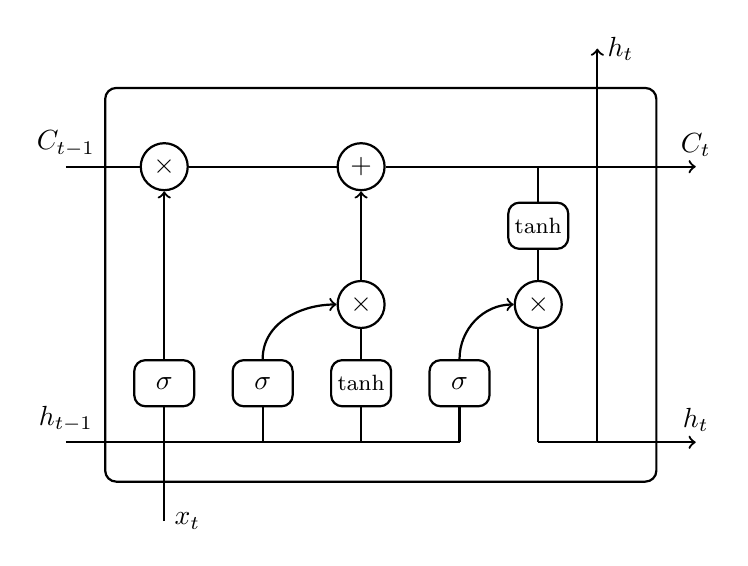
\begin{tikzpicture}[thick]
    % Unit
    \draw [rounded corners, thick] (0, 0) rectangle (7, 5);

    % Conveyor Belt
    \path (0.75, 4) coordinate [draw, circle, thick, inner sep=6pt]
          (m1) node {$\times$};
    \path (3.25, 4) coordinate [draw, circle, thick, inner sep=6pt]
          (add) node {$+$};
    \draw [thick, ->]
          (-0.5, 4) node [above] {$C_{t-1}$}
       -- (m1)
       -- (add)
       -- (7.5, 4) node [above] {$C_t$};

    % previous activation input
   \path (-0.5, 0.5) coordinate (hp) node [above] {$h_{t-1}$};

    % input
    \path (0.75, -0.5) coordinate (x) node [right] {$x_t$};

    % output
    \path (6.25, 5.5) coordinate (h1) node [right] {$h_t$};

    \path (7.5, 0.5) coordinate (h2) node [above] {$h_t$};

    % forget gate
    \path (0.75, 1.25) coordinate
          [draw, rectangle, rounded corners, thick, text width=15pt, text height=10pt]
          (fg);
    \draw (fg) node {$\sigma$};
    \coordinate (a1) at (0.75, 0.5);

    % input gate
    \path (2, 1.25) coordinate
          [draw, rectangle, rounded corners, thick, text width=15pt, text height=10pt]
          (ig);
    \draw (ig) node {$\sigma$};
    \coordinate (a2) at (2, 0.5);

    % Activation function
    \path (3.25, 1.25) coordinate
          [draw, rectangle, rounded corners, thick, text width=15pt, text height=10pt]
          (f1);
    \draw (f1) node {\footnotesize$\tanh$};
    \coordinate (a3) at (3.25, 0.5);

    \path (f1)+(0, 1) coordinate [draw, circle, thick, inner sep=6pt]
          (m2) node {$\times$};

    % output gate
    \path (4.5, 1.25) coordinate
          [draw, rectangle, rounded corners, thick, text width=15pt, text height=10pt]
          (og);
    \draw (og) node {$\sigma$};
    \coordinate (a4) at (4.5, 0.5);

    % Output activation
    \path (5.5, 3.25) coordinate
          [draw, rectangle, rounded corners, thick, text width=15pt, text height=10pt]
          (f2);
    \draw (f2) node {\footnotesize$\tanh$};
    \coordinate (a5) at (5.5, 4);
    \coordinate (a6) at (5.5, 0.5);
    \coordinate (a7) at (6.25, 0.5);

    \path (f2)+(0, -1) coordinate [draw, circle, thick, inner sep=6pt]
          (m3) node {$\times$};

    % Connections
    \draw (hp) -- (a1) -- (a2) -- (a3) -- (a4);
    \draw (x) -- (a1);

    % Forget gate
    \draw (a1) -- (fg);
    \draw [->] (fg) -- (m1);

    % Input gate
    \draw (a2) -- (ig);

    % Input activation
    \path [->] (ig) edge [out=90, in=180] (m2);
    \draw (a3) -- (f1);
    \draw (f1) -- (m2);
    \draw [->] (m2) -- (add);

    % Output gate
    \draw (a4) -- (og);
    \path [->] (og) edge [out=90, in=180] (m3);

    % Output activation
    \draw (a5) -- (f2);
    \draw (f2) -- (m3);
    \draw (m3) -- (a6);
    \draw (a6) -- (a7);
    \draw [->] (a7) -- (h1);
    \draw [->] (a7) -- (h2);

  \end{tikzpicture}
\end{slide}

\begin{slide}{LSTMs}
  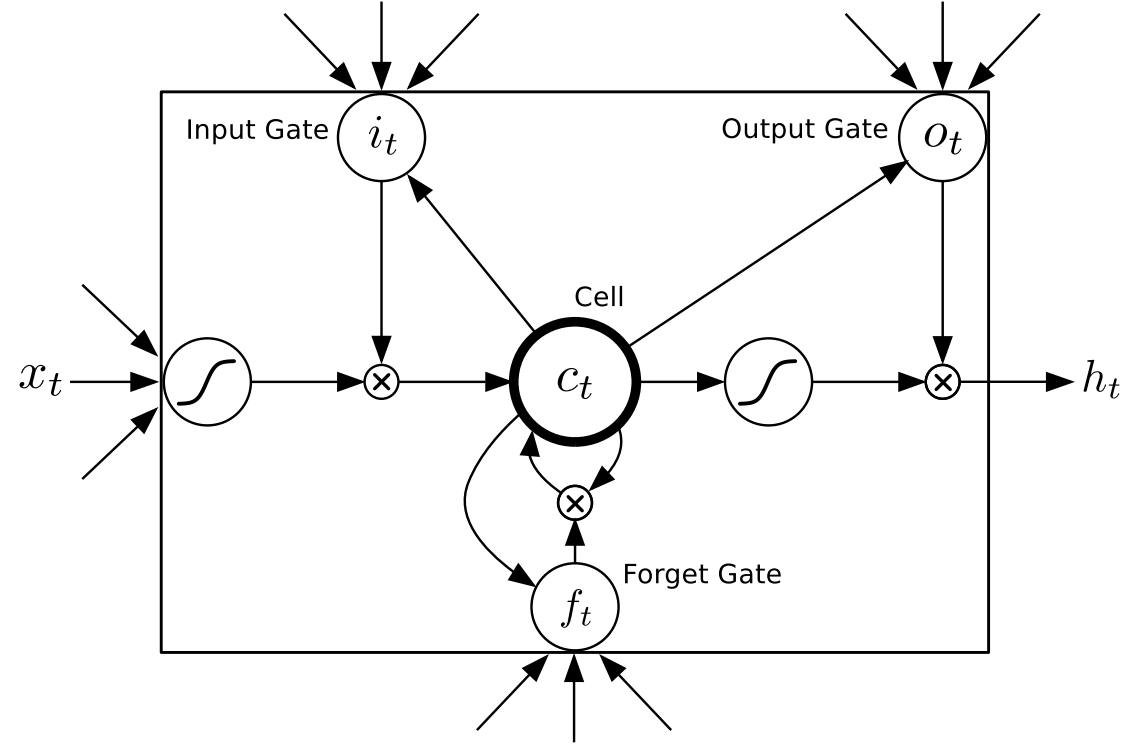
\includegraphics[scale=0.5]{lstm};
\end{slide}

\begin{slide}{LSTMs: What can they do?}
  \frameheader{So, what can LSTMs actually do?}
\end{slide}

\begin{slide}{LSTMs: What can they do?}
  % trained an LSTM of Leo Tolstoy’s War and Peace and then generated samples every 100 iterations of training
  % Understands that words are delimited by spaces
  \begin{quote}
    tyntd-iafhatawiaoihrdemot  lytdws  e ,tfti, astai f ogoh eoase rrranbyne 'nhthnee e plia tklrgd t o idoe ns,smtt   h ne etie h,hregtrs nigtike,aoaenns lng
  \end{quote}
  \vspace{0.25cm}
  Iteration: 100
\begin{flushleft}\cite{lstm}\end{flushleft}
\end{slide}

\begin{slide}{LSTMs: What can they do?}
  % quotes, peridos
  \begin{quote}
    ``Tmont thithey'' fomesscerliund
      Keushey. Thom here
      sheulke, anmerenith ol sivh I lalterthend Bleipile shuwy fil on aseterlome
      coaniogennc Phe lism thond hon at. MeiDimorotion in ther thize."
  \end{quote}
  \vspace{0.25cm}
  Iteration: 300
\begin{flushleft}\cite{lstm}\end{flushleft}
\end{slide}

\begin{slide}{LSTMs: What can they do?}
  % real words
  \begin{quote}
    we counter. He stutn co des. His stanted out one ofler that concossions and was to gearang reay Jotrets and with fre colt otf paitt thin wall. Which das stimn
  \end{quote}
  \vspace{0.25cm}
  Iteration: 500
\begin{flushleft}\cite{lstm}\end{flushleft}
\end{slide}

\begin{slide}{LSTMs: What can they do?}
  % more real words
  \begin{quote}
    Aftair fall unsuch that the hall for Prince Velzonski's that me of
    her hearly, and behs to so arwage fiving were to it beloge, pavu say falling misfort
    how, and Gogition is so overelical and ofter.
  \end{quote}
  \vspace{0.25cm}
  Iteration: 700
\begin{flushleft}\cite{lstm}\end{flushleft}
\end{slide}

\begin{slide}{LSTMs: What can they do?}
  % more real words
  \begin{quote}
    ``Why do what that day,'' replied Natasha, and wishing to himself the fact the princess, Princess Mary was easier, fed in had oftened him. Pierre aking his soul came to the packs and drove up his father-in-law women.
  \end{quote}
  \vspace{0.25cm}
  Iteration: 2000
\begin{flushleft}\cite{lstm}\end{flushleft}
\end{slide}

\begin{slide}{LSTMs: What can they do?}
  {
    \huge
    They can write Linux kernel code!
  }
\end{slide}
